\documentclass[conference]{IEEEtran}
\IEEEoverridecommandlockouts

\usepackage{cite}
\usepackage{amsmath,amssymb,amsfonts}
\usepackage{algorithmic}
\usepackage{graphicx}
\usepackage{textcomp}
\usepackage{xcolor}
\usepackage{hyperref}
\usepackage{listings}
\lstset{
  language=C++,
  basicstyle=\ttfamily\footnotesize,
  keywordstyle=\color{blue},
  commentstyle=\color{gray}\itshape,
  stringstyle=\color{red},
  numbers=none,
  numbersep=5pt,
  frame=single,
  breaklines=true,
  breakatwhitespace=true,
  postbreak=\mbox{\textcolor{gray}{$\hookrightarrow$}\space},
  showstringspaces=false,
  captionpos=b,
  tabsize=2
}


\def\BibTeX{{\rm B\kern-.05em{\sc i\kern-.025em b}\kern-.08em
    T\kern-.1667em\lower.7ex\hbox{E}\kern-.125emX}}

\begin{document}

\title{Design and Implementation of a Line Following and Obstacle Avoidance Robot}

\author{
\IEEEauthorblockN{Your Name\IEEEauthorrefmark{1}, Student 2\IEEEauthorrefmark{1}, Student 3\IEEEauthorrefmark{1}, Student 4\IEEEauthorrefmark{1}}
\IEEEauthorblockA{\IEEEauthorrefmark{1}Systems Engineering and Prototyping, BSc Electronic Engineering\\
Hochschule Hamm-Lippstadt, Lippstadt, Germany\\
\{your.name, student2, student3, student4\}@stud.hshl.de}
}

\maketitle

\begin{abstract}
This paper presents the.
\end{abstract}

\begin{IEEEkeywords}
Line follower robot,
\end{IEEEkeywords}

\section{Introduction}
This project focuses on the development of a simple mobile robot that can autonomously follow a black line on a white surface and avoid obstacles placed in its path. The robot uses infrared sensors to detect the line and an ultrasonic sensor to detect nearby objects. An Arduino microcontroller is used to process sensor inputs and control motors accordingly.


\section{System Design and Engineering}
The design of the robot was developed based on the tasks and milestones defined at the beginning of the project. These included line following, obstacle detection and avoidance, and integration of all components into a working prototype. It uses two infrared (IR) sensors to detect the black line and an ultrasonic sensor to measure the distance from obstacles. These sensors send signals to an Arduino Uno, that acts as the main controller.

The Arduino processes data and decides how the system should respond: either adjusting its path to stay on the line or stopping and maneuvering around an obstacle. Movement is handled by two DC motors controlled through an L298N motor driver.

Power is provided by a 9V battery pack, with regulation to supply the required voltages for the microcontroller and sensors. A simplified block diagram of the system is shown in Fig.~\ref{fig:block}
\begin{figure}[h]
    \centering
    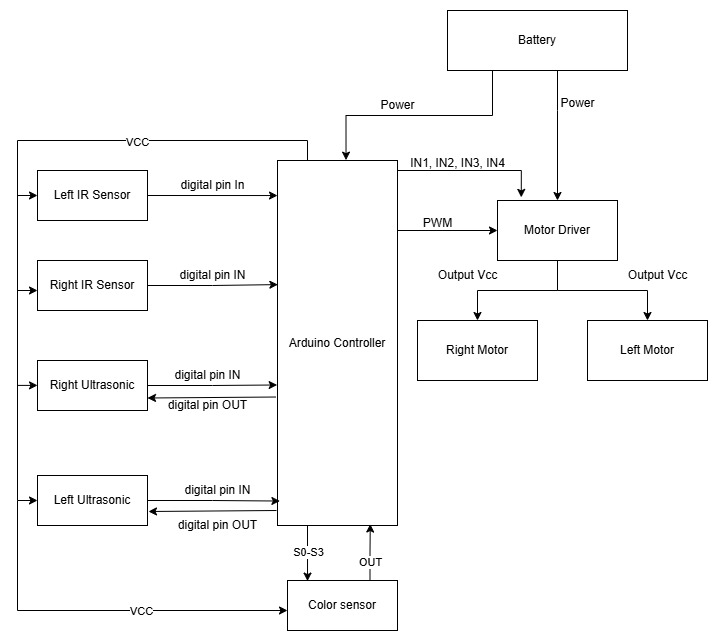
\includegraphics[width=0.5\linewidth]{block_diagram.jpg}
    \caption{Block diagram of the robot system architecture.}
    \label{fig:block}
\end{figure}

\section{Prototyping and Design}

\subsection{Electronic Components}

\subsection{Virtual and Physical Prototypes}


\subsection{Hardware Assembly}
All components were mounted on a chassis and connected as per the schematic.

\section{Circuit Design}
%\begin{itemize}
 %   \item The schematic includes sensors, motor driver, Arduino, and power source.
  %  \item Wiring includes proper voltage connections and pin mappings for sensors and motors.
%\end{itemize}

\begin{figure}[htbp]
\centerline{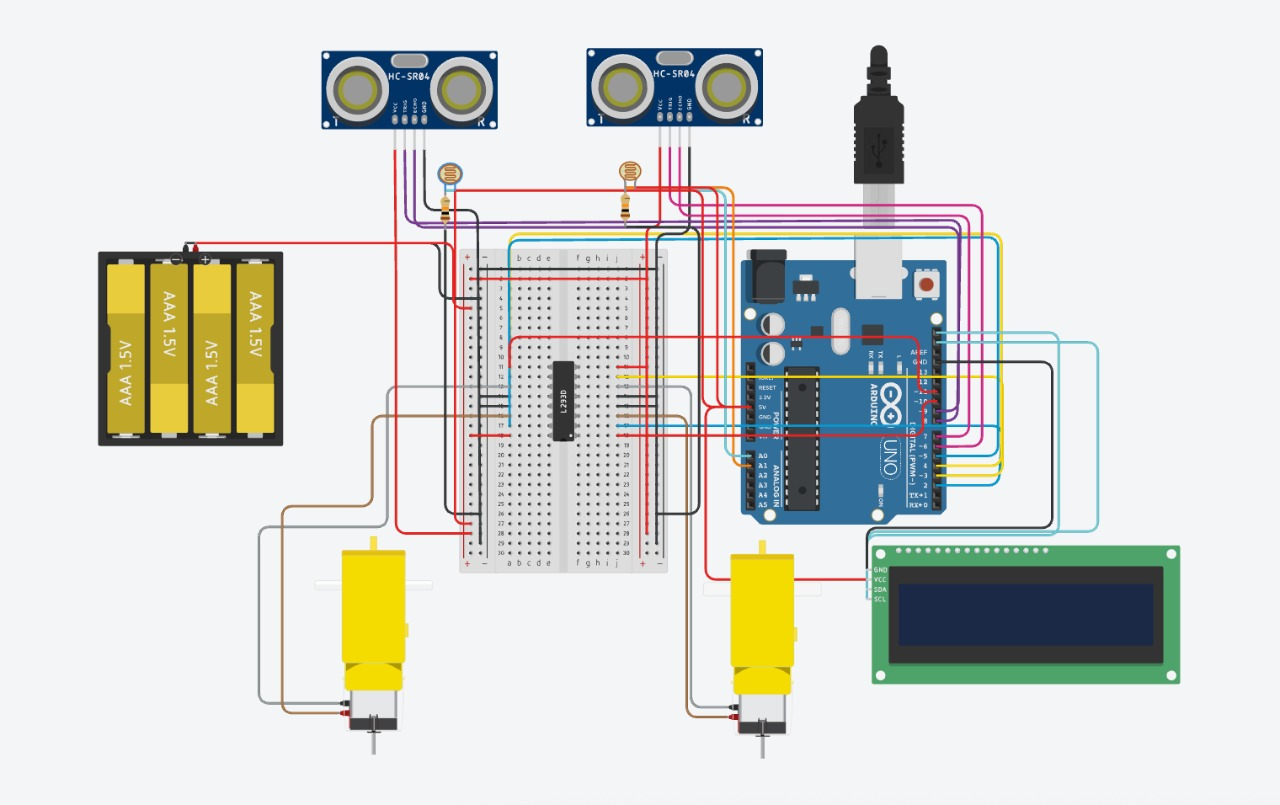
\includegraphics[width=0.9\linewidth]{circuit_diagram.jpg}}
\caption{Complete circuit layout of the robot}
\label{fig:circuit}
\end{figure}

\section{Software Implementation}
\label{soft}

\subsection{Initialization of Sensors and Actuators}
\subsubsection*{1. Sensors Initialization}

\paragraph{Ultrasonic Sensors (Left/Right)}
Pins for the ultrasonic sensors are defined in the file 'UltrasonicSensor.h'. They are set up and initialized in the 'UltrasonicSensor.cpp' and 'main.cpp' files. Relevant snippets are shown below:


\begin{lstlisting}[language=C++, caption=Pin definitions in UltrasonicSensor.h]
// Ultrasonic sensor pin definitions
#define LEFT_TRIG_PIN 8
#define LEFT_ECHO_PIN 9
#define RIGHT_TRIG_PIN 6
#define RIGHT_ECHO_PIN 7
\end{lstlisting}

\begin{lstlisting}[language=C++, caption=Pin setup in UltrasonicSensor.cpp]
// Set trigger as output and echo as input
void UltrasonicSensor::begin() {
   pinMode(trigPin, OUTPUT);
   pinMode(echoPin, INPUT);
}
\end{lstlisting}

\begin{lstlisting}[language=C++, caption=Sensor initialization in main.cpp]
// Create hardware instances
...
UltrasonicSensor rightUltrasonic(
  RIGHT_TRIG_PIN,
  RIGHT_ECHO_PIN);
UltrasonicSensor leftUltrasonic(
  LEFT_TRIG_PIN,
  LEFT_ECHO_PIN);
RobotNavigation robotNav(
  &rightUltrasonic,
  &leftUltrasonic,
  &motor);
 
// Initialize ultrasonic sensors
void setup() {
   ...
   rightUltrasonic.begin();
   leftUltrasonic.begin();
   ...
}
\end{lstlisting}

\paragraph{IR Sensors (Left/Right)}

Pins for the IR sensors are defined in 'RobotNavigation.h' and initialized in 'RobotNavigation.cpp' and in 'main.cpp'. Relevant snippets are shown below:

\begin{lstlisting}[language=C++, caption=IR sensor pin definitions in RobotNavigation.h]
// Line sensor digital pins
#define LINE_SENSOR_LEFT 13
#define LINE_SENSOR_RIGHT 12
\end{lstlisting}

\begin{lstlisting}[language=C++, caption=IR sensor pin initialization in RobotNavigation.cpp]
void RobotNavigation::begin() {
  pinMode(LINE_SENSOR_LEFT, INPUT);
  pinMode(LINE_SENSOR_RIGHT, INPUT);
}
\end{lstlisting}

\begin{lstlisting}[language=C++, caption=IR sensor pin initialization in main.cpp]
void setup() {
  ...
  // Start navigation system
  robotNav.begin();
}
\end{lstlisting}

\paragraph{Color Sensor}

Pins for the color sensor are defined in 'ColorSensor.h' and initialized in 'ColorSensor.cpp'. Relevant snippets are shown below:

\begin{lstlisting}[language=C++, caption=Color sensor pin definitions in ColorSensor.h]
// Pin definitions
#define COLOR_SENSOR_OUTPUT_FREQUENCY_INPUT_S0 A0
#define COLOR_SENSOR_OUTPUT_FREQUENCY_INPUT_S1 A1
#define COLOR_SENSOR_PHOTODIODE_INPUT_S2 A2
#define COLOR_SENSOR_PHOTODIODE_INPUT_S3 A3
#define COLOR_SENSOR_OUTPUT_PIN A4
\end{lstlisting}

\begin{lstlisting}[language=C++, caption=Color sensor pin initialization in ColorSensor.cpp]
void ColorSensor::ColorSensorInit() {
    pinMode(
      COLOR_SENSOR_OUTPUT_FREQUENCY_INPUT_S0,
      OUTPUT);
    pinMode(
      COLOR_SENSOR_OUTPUT_FREQUENCY_INPUT_S1,
      OUTPUT);
    pinMode(
      COLOR_SENSOR_PHOTODIODE_INPUT_S2,
      OUTPUT);
    pinMode(
      COLOR_SENSOR_PHOTODIODE_INPUT_S3,
      OUTPUT);
    pinMode(
      COLOR_SENSOR_OUTPUT_PIN,
      INPUT);

    digitalWrite(
      COLOR_SENSOR_OUTPUT_FREQUENCY_INPUT_S0,
      HIGH); // Full scale
    digitalWrite(
      COLOR_SENSOR_OUTPUT_FREQUENCY_INPUT_S1,
      LOW); // Frequency scaling = 20%
}
\end{lstlisting}

\subsubsection*{2. Actuators (Motors) Initialization}
Motor Control Pins are defined in the file 'MotorControl.h'. Their setup and initialization are made in the 'main.cpp' file. Relevant snippets are shown below:

\begin{lstlisting}[language=C++, caption=Pin definitions in MotorControl.h]
// Motor control pin definitions
#define LEFT_MOTOR_SPEED_PIN 10
#define RIGHT_MOTOR_SPEED_PIN 11
#define LEFT_MOTOR_FORWARD_PIN 2
#define LEFT_MOTOR_BACKWARD_PIN 3
#define RIGHT_MOTOR_FORWARD_PIN 4
#define RIGHT_MOTOR_BACKWARD_PIN 5
\end{lstlisting}

\begin{lstlisting}[language=C++, caption=Pins initialization in main.cpp]
// Create hardware instances
MotorControl motor;
..

RobotNavigation robotNav(
  &rightUltrasonic,
  &leftUltrasonic,
  &motor
);
// Arduino initialization
void setup() {
  // Setup motor pins as outputs
  pinMode(LEFT_MOTOR_SPEED_PIN, OUTPUT);
  pinMode(RIGHT_MOTOR_SPEED_PIN, OUTPUT);
  pinMode(LEFT_MOTOR_FORWARD_PIN, OUTPUT);
  pinMode(LEFT_MOTOR_BACKWARD_PIN, OUTPUT);
  pinMode(RIGHT_MOTOR_FORWARD_PIN, OUTPUT);
  pinMode(RIGHT_MOTOR_BACKWARD_PIN, OUTPUT);
  ...
}
\end{lstlisting}

\subsubsection*{Key Initialization Features}
\begin{enumerate}
  \item \textbf{Pin Abstraction}
    \begin{itemize}
      \item Hardware pins are abstracted via \verb|#define| macros.
      \item Logical separation of sensor and actuator types.
    \end{itemize}
  \item \textbf{Modular Initialization}
    \begin{itemize}
      \item Each sensor type has its own initialization routine.
      \item Motor control setup is centralized in \texttt{main.cpp}.
    \end{itemize}
  \item \textbf{Hardware–Software Mapping}
    \begin{itemize}
      \item See Fig.~1. Block diagram of the robot system architecture.
    \end{itemize}
\end{enumerate}

This summary ensures the reader understands the overarching design—pin abstraction, modular setup, mapping, and your carefully ordered startup sequence—before diving into higher‑level behavior logic.


\subsection{Movement Control Algorithms}

\subsubsection*{Core Movement Functions}
We implement four basic motion primitives in 'MotorControl.cpp'.

\subsection{Behavioral Decision Logic}


\section{Git Usage and Collaboration}
Project development was tracked using GitHub. Each member's contribution should be explained.

\begin{table}[ht]
\centering
\begin{tabular}{l|c}
\hline
\textbf{Team Member} & \textbf{Number of Commits} \\
\hline
Your Name     & 77 \\
Student 2     & 25 \\
Student 3     & 9  \\
Student 4     & 3  \\
\hline
\textbf{Total} & \textbf{114} \\
\hline
\end{tabular}
\caption{GitHub Commits by Team Members}
\label{table:commit}
\end{table}

\section{Key Achievements}


\section*{Acknowledgment}

\begin{thebibliography}{00}
\bibitem{arduino} Arduino Documentation. \url{https://www.arduino.cc/en/Guide}
\bibitem{tinkercad} Tinkercad Simulation. \url{https://www.tinkercad.com}
\bibitem{uppaal} Uppaal Model Checker. \url{http://www.uppaal.org/}
\end{thebibliography}

\section*{Declaration of Originality}
We hereby declare that this report is our own work and that we have acknowledged all sources used.

\end{document}
